\documentclass[man]{apa2}
\usepackage{pslatex}
\usepackage{amssymb}
\usepackage{graphicx}
\usepackage{color}
\usepackage{covington}
\usepackage[usenames,dvipsnames]{xcolor}
\usepackage{booktabs}
\usepackage{setspace}

\title{The trouble with quantifiers: Children's difficulty with scalar terms extends beyond the realm of implicatures}

\threeauthors{Alexandra C. Horowtiz}{Rose M. Schneider}{Michael C. Frank}
\threeaffiliations{Department of Psychology, Stanford University}{Department of Psychology, Stanford University}{Department of Psychology, Stanford University}

\abstract{Are the forms of words systematically related to their meaning? The arbitrariness of the sign has long been a foundational part of our understanding of human language. Theories of communication predict a relationship between length and meaning, however: Longer descriptions should be more conceptually complex. Here we show that both the lexicons of human languages and individual speakers encode the relationship between linguistic and conceptual complexity. Experimentally, participants mapped longer words to more complex objects in comprehension and production tasks and across a range of stimuli. Explicit judgments of conceptual complexity were also highly correlated with implicit measures of study time in a memory task, suggesting that complexity is directly related to basic cognitive processes. Observationally, judgments of conceptual complexity for a sample of real words correlate highly with their length across 80 languages, even controlling for frequency, familiarity, imageability, and concreteness. While word lengths are systematically related to usage---both frequency and contextual predictability---our results reveal a systematic relationship with meaning as well. They point to a general regularity in the design of lexicons and suggest that pragmatic pressures may influence the structure of the lexicon.

~\\

Keywords: communication, lexicon, language evolution}

\shorttitle{The trouble with quantifiers}
\rightheader{The trouble with quantifiers}

\acknowledgements{ We gratefully acknowledge. 

~\\

\noindent Address all correspondence to Rose M. Schneider, Stanford University, Department of Psychology, Jordan Hall, 450 Serra Mall (Bldg. 420), Stanford, CA, 94305. Phone: 650-721-9270. E-mail: \texttt{rschneid@stanford.edu}.}

\begin{document}

\maketitle               

\section{Introduction}
Why are implicatures important? 

What are the developmental differences?

Why is this interesting?

What are some of the sources of difficulty with children understanding implicatures? 

Stiller et al. 

Previous studies examine implicatures using differing methods, and the results are difficult to compare

Introduce new paradigm for adhoc and scalar implicature research 


\subsection{Previous work}

In study 1, we should that one paradigm provides reliable and consistent measurement of implicature performance in children 3-5; however, children succeed with ad hocs, but have difficulty with scalar items; given that children were successful in computing ad hoc implicatures with this paradigm, could the poor performance in these scalar trials be due to the fact that the trials were intermixed with the adhoc trials?

In study 2, we examined this possibility by only testing scalar items, and found that while this increased performance for older children, children were still having difficulty with this task, particularly with the ?some? and ?none? trials

Children who had problems with ?some? were also more likely to have issues with ?none? 

There are several reasons we might have seen the results that we did

Children may need to know both ends of the quantifier scale in order to be able to make an implicature

There might be problems with inhibition; children in these trials might listening through the quantifier and answering purely based on the target noun; this is supported by the fact that children reliably choose ?all? for ``some'' and ``none'' trials

Do children not know what these quantifiers mean?

\subsection{Current work}

In study three, we explored these alternatives by running children on both the SI task, an inhibitory control task (DCCS) as well as the Give-Quantifier task, a productive measure of quantifier knowledge

Interestingly, we found that the patterns of performance persist in SI as in Horowitz and Frank, and that DCCS was not predictive of performance in either SI or GQ when controlled for age

However, we found correlations between the Give-Quantifier task with ?some? and ?none? trials (except for GQ none and SI some, I think) when controlling for age; this seems to indicate that difficulties with these scalar terms exist outside of the implicature realm

Children just seem to have a trouble with quantifiers


\section{Experiment 1: Ad hoc and scalar implicature computation in children}

Given the difficulty in equating results on children's computation of implicatures across different methods and paradigms, we created a single task that could be adapted to investigate both ad hoc and scalar items in one task. This task involved one set of stimuli presented in the same order to all participants; however, the particular items queried were counterbalanced across participants. Thus, with one set of stimuli we created a novel paradigm wherein we could directly compare children's performance on both ad hoc and scalar implicatures in a single experimental session. In Experiment 1, we included questions about ad hoc and scalar implicatures within one session, and found that this paradigm was appropriate for ad hoc items, but children still experienced difficulty computing scalar items. In Experiment 2, we included only scalar items in the task, and found that participants were moderately more successful at making implicatures when these trials were presented in isolation. In Experiment 3, we explored two alternatives potentially driving children's difficulties in this task.  

\subsection{Methods}

\subsubsection{Participants} A planned sample of 48 children was recruited from Bing Nursery School at Stanford University. These children were drawn from two age groups: twenty-four 4.0 -- 4.5-year-olds (M = 4;2, median = 4.19, SD = 0.14) and 24 4.5 -- 5.0-year-olds (M = 4.74, median = 4.73, SD = .16). Two children were excluded from the final sample for not completing the task, and one additional child was excluded due to experimenter error. The final sample was comprised of (XX males and XX females) with English as their primary language. Across all experiments, no child completed more than one session of the task. 

\begin{figure} 
 \begin{center} 
  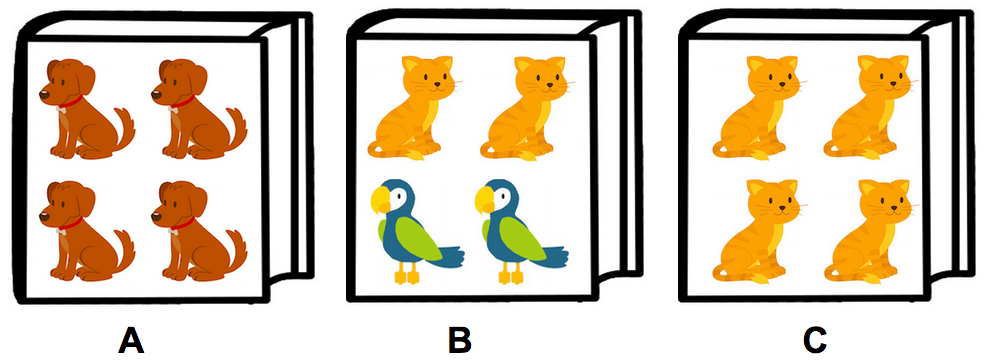
\includegraphics[height=2in]{figures/implicatures_demo_letters.png} 
  \caption{\label{fig:demo} Example trial stimuli used in all experiments. Children received a clue from the experimenter about which book she had in mind and responded based solely on the clue; this was either an ad hoc or a scalar description of a book with either an unambiguous or implicature target.} 
 \end{center} 
\end{figure}	 

\subsubsection{Stimuli}
Stimuli for all experiments were created to be appropriate for questions about both ad hoc and scalar implicatures, allowing the experimenter to use one set of stimuli for both kinds of items in one experimental session. Therefore, we created a set of printed pictures of three book covers with four familiar items on each cover. In each trial, one book cover contained four items of the same kind (e.g., four cats), another book cover contained four items of another kind (e.g., dogs), and the final cover contained two items of a new set and two items repeated from one of the other book covers (e.g., two birds and two cats). An example of the stimuli can be seen in Figure \ref{fig:demo}. Experiment 1 consisted of 18 test trials preceded by one test trial, with three book covers with only one familiar item on each. All items on the book covers were familiar to children, and were able to be identified. All participants saw the same book covers in the same order. 


\subsubsection{Procedure}
Participants were tested in individual sessions in a quiet room at their nursery school. The experimenter introduced the study as a guessing game, and explained that the child would receive one hint about which book cover the experimenter had in mind. In the instructions for the task, the experimenter emphasized that the child would only receive one clue about what book the experimenter was describing, and they had to use that clue to make their decision. All participants saw the same book covers in the same order; however, (three?) scripts were counterbalanced across participants so that all items were 

\subsection{Results and Discussion}



\section{Experiment 2: Mapping Task (Artificial Objects)}


\subsection{Methods}
\subsubsection{Participants} 
\subsubsection{Stimuli}

\subsubsection{Procedure}


\subsection{Results and Discussion}

				
\section{Experiment 3: Control Mapping Task (Artificial Objects)}

\subsection{Methods}
\subsubsection{Participants} 200 participants completed the experiment.
\subsubsection{Stimuli} h

\subsubsection{Procedure}
h

\subsection{Results and Discussion}
h

\section{General Discussion}

h




\bibliographystyle{apacite2}
\bibliography{biblibrary}

\newpage
\theappendix 

\section{}

\end{document}